\documentclass[12pt,spinewidth=25mm,coverwidth=15cm,coverheight=20cm,%flapwidth=6cm,
bgtikznodes]{bookcover}
\usepackage{contour,lipsum}
\contourlength{1pt}
\definecolor{lightbrown}{RGB}{176,88,0}
\colorlet{title}{white!60!black}
\begin{document}

% Black background color on the whole cover
\setbookcover{bgcolor}{whole}{color=black}

% Brown background picture on the whole cover, without the flaps
% \setbookcover{bgpic}{whole without flaps}{./figures/bg.jpg}

% Vertical light brown transparent trails on the back cover by a tikz code
% \setbookcover{bgtikz}{back}{
%     \fill[opacity=0.3,color=lightbrown] 
%     (0mm,0mm) rectangle (20mm,210mm) (100mm,0mm) rectangle (150mm,210mm);}

% Vertical light brown transparent trails on the front cover by a tikz code
% \setbookcover{bgtikz}{front}{
%     \fill[opacity=0.3,color=lightbrown] 
%     (0mm,0mm) rectangle (50mm,210mm) (130mm,0mm) rectangle (150mm,210mm);}

% Remark
\setbookcover{fgfirst}{above front}{
    \color{blue} Protopopov 1996--1999 | \textsc{Tratado}}

% Text on the front cover
\setbookcover{fgfirst}{front}{
    \centering
    \vspace{25mm}
    \color{title}\sffamily\bfseries
    \resizebox*{50mm}{8mm}{\contour[120]{black}{Anatoliy Protopopov}}
    \par
    \vspace{10mm}
    \resizebox*{90mm}{40mm}{\parbox{35mm}{
        \centering
        \contour[120]{black}{\textsc{tratado sobre}}\\
        \contour[120]{black}{\textsc{el amor}}\\}}}

% Picture (cards.png) on the front, behind the title
\setbookcover{fgsecond}{front}{
    \vspace{70mm}
    \centering
    \includegraphics[width=\textwidth]{./figures/1-peacock-dean-nahum-unsplash-4226.jpg}}  

% Text on the spine
\setbookcover{fgfirst}{spine}{
    \vfill
    \centering
    \rotatebox[origin=c]{90}{\contour[120]{black}{
        \color{title}\huge\sffamily\bfseries 
        Anatoliy Protopopov | \textsc{Tratado Sobre el Amor}}}
    \vfill}

% % % % % Text on the back cover
\setbookcover{fgfirst}{back}{
    \centering
    \vspace{20mm}
    \parbox{110mm}{\color{white}
    \lipsum[3-4]
    }}

% Text and picture (dice.png) on the front flap
% % % % \setbookcover{fgfirst}{front flap}{
% % % %     \centering
% % % %     \vspace{20mm}
% % % %     \parbox{40mm}{\color{white}\lipsum[2]}
% % % %     \vfill
% % % %     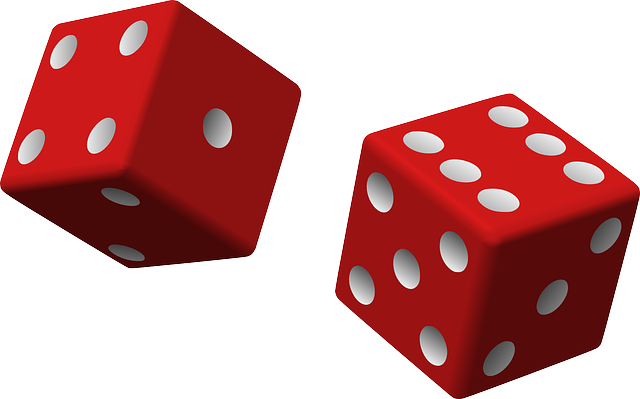
\includegraphics[width=30mm]{./figures/dice.png}
% % % %     \vspace{10mm}}

% Text on the back flap
% % % % \setbookcover{fgfirst}{back flap}{
% % % %     \centering
% % % %     \vspace{20mm}
% % % %     \parbox{40mm}{\color{white}\lipsum[2]}}

% Making the dust jucket
\makebookcover

\end{document} 